\documentclass[letterpaper]{article}
\usepackage[utf8]{inputenc}
\usepackage[spanish, mexico]{babel}
\usepackage{amssymb, amsmath}
\usepackage{graphicx}
\usepackage[margin=1.5cm,
vmargin={1.5cm,0.7cm},
includefoot]{geometry}
\usepackage{amsthm}
\usepackage{dsfont}
\usepackage{mathtools}
\usepackage{graphicx}

\providecommand{\abs}[1]{\left|#1\right|}

\newtheorem*{remark}{Recuerde}

\newcommand{\tq}{ \quad \cdot  \backepsilon \cdot \quad }

\newcommand{\R}{\mathds{R}}

\renewcommand{\*}{\cdot}

\newtheorem{theorem}{Teorema}[]
\theoremstyle{definition}
\newtheorem{definition}{Definición}

\begin{document}

\setlength{\unitlength}{1cm}
\thispagestyle{empty}
\begin{picture}(19,3)
\put(-0.5,1.2){
\includegraphics[scale=.20]{img/unam1.png}}
\put(16,1){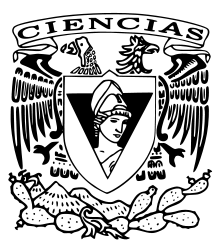
\includegraphics[scale=.29]{img/fciencias1.png}}
\end{picture}

\begin{center}
	\vspace{-114pt}
	\textbf{\large Matemáticas para las Ciencias II}\\
	\textbf{ Semestre 2020-2}\\
	Prof. Pedro Porras Flores\\
	Ayud. Irving Hernández Rosas \\
	\textbf{Tarea Examen III}\\[0.15cm]
	Kevin Ariel Merino Peña\footnote{Número de cuenta 317031326} Armando Abraham Aquino Chapa\footnote{Número de cuenta n}
	José Manuel Pedro Méndez\footnote{Número de cuenta n}\\ [0.12cm]
	\today
\end{center}
\vspace{-10pt}
\rule{19cm}{0.3mm}

\noindent \textbf{Instrucciones:} Realice las siguientes ejercicios escribiéndolos  de manera clara, los puede realizar en \LaTeX, en un cuaderno etc, pero debe de subir el archivo en la sesión de classrroom en formato pdf para su revisión.

%\section*{La integral}

\begin{enumerate}

% -----------------------------------------------------
% Problema uno
% -----------------------------------------------------


\section*{Métodos de integración}

\subsection*{Integración por partes (2.5 pts.)}
\item Realice las siguientes integrales:
\begin{enumerate}
	\item$\displaystyle \int x \sin(x) \, dx$
	\begin{align*}
		f &= x & df &= dx\\
		g &= -\cos(x) & dg &= \sin(x)dx
	\end{align*}
	\begin{align*}
		&= f \* g - \int g\*df &&\text{Empleando integración por partes}\\
		&= x(-\cos(x)) - \int -\cos(x)dx &&\text{Reemplazando con los valores elegidos}\\
		&= -x\cos(x) + \int \cos(x)dx &&\text{Porque la integral es un operador lineal}\\
		&= -x\cos(x) + \sin(x) &&\text{La integral de }\cos(x) = \sin(x)
	\end{align*}
	\[ \therefore \int x \sin(x) \, dx = \sin(x) - x\cos(x) + C, C \in \R  \]
	
	\item$\displaystyle \int x^2 e^x \, dx$
	\begin{align*}
		f &= x^2 & df &= 2x dx\\
		g &= e^x & dg &= e^xdx
	\end{align*}
	\begin{align*}
		&= f \* g - \int g\*df &&\text{Empleando integración por partes}\\
		&= x^2 \* e^x - \int e^x \* 2xdx &&\text{Haciendo uso de las funciones elegidas}\\
		&= e^x x^2 -2\underbrace{\int xe^xdx}_\text{Otra integral} &&\text{Sacando escalares por la linealidad de la integral}
	\end{align*}
	\[ \int xe^xdx = \]
	\begin{align*}
		f &= x & df &= dx\\
		g &= e^x & dg &= e^xdx
	\end{align*}
	\begin{align*}
		&= f \* g - \int g\*df &&\text{Empleando integración por partes}\\
		&= x\* e^x - \int e^x \*dx &&\text{Haciendo uso de las funciones elegidas}\\
		&= xe^x - e^x &&\text{Conocemos de Mate I la integral de }e\\
		&= e^x(x - 1)\\
	\end{align*}
	\begin{align*}
		e^x x^2 -2\int xe^xdx &= e^x x^2 -2e^x(x-1) &&\text{Reemplazando en el resultado anterior}\\
		&= e^x(x^2 -2(x-1)) &&\text{Factorizando}
	\end{align*}
	\[ \therefore \int xe^xdx = e^x(x^2 -2(x-1)) + C, C \in \R \]
	
	\item$\displaystyle \int x^2 \sin(x) \, dx$
	\begin{align*}
		f &= x^2 & df &=2x\,dx \\
		g &= -\cos(x) & dg &= \sin(x)dx
	\end{align*}
	\begin{align*}
		&= f \* g - \int g\,df &&\text{Empleando integración por partes}\\
		&= -x^2\cos(x) - \int -\cos(x)2x\,dx &&\text{Haciendo uso de las funciones elegidas}\\
		&= -x^2\cos(x) + \underbrace{2\int x\cos(x)dx}_\text{Integración por partes} &&\text{Sabemos que la integral es un operador lineal}
	\end{align*}
	\[ \int x\cos(x)dx = \]
	\begin{align*}
		f &= x & df &=dx \\
		g &= \sin(x) & dg &= \cos(x)dx
	\end{align*}
	\begin{align*}
		&= f \* g - \int g\,df &&\text{Empleando integración por partes}\\
		&= x\sin(x) - \int \sin(x)\,dx &&\text{Haciendo uso de las funciones elegidas}\\
		&= x\sin(x) - (-\cos(x)) &&\text{De Mate I conocemos las integrales de las f. trigonométricas}\\
		&= x\sin(x) + \cos(x) &&\text{Operando signos}
	\end{align*}
	\begin{align*}
		\int x^2 \sin(x) \, dx &= -x^2\cos(x) + 2\int x\cos(x)dx &&\text{Reemplazando en el resultado anterior}\\
		&= -x^2\cos(x) + 2(x\sin(x) + \cos(x)) &&\text{Factorizando }\\
		&= \cos(x)(2 -x^2) +2x\sin(x) &&\text{ }
	\end{align*}
	\[ \therefore 	\int x^2 \sin(x) \, dx = \cos(x)(2 -x^2) +2x\sin(x)  + C, C \in \R \]
	 \newpage
	\item$\displaystyle \int x \ln(x) \, dx$
	\begin{align*}
		f &= \ln(x) & df &=\frac{1}{x}dx \\
		g &= \dfrac{x^2}{2} & dg &= xdx
	\end{align*}
	\begin{align*}
		&= f \* g - \int g\,df &&\text{Empleando integración por partes}\\
		&= \dfrac{x^2\ln(x)}{2} - \int \dfrac{x^2}{2}\dfrac{1}{x}\,dx && \text{Reemplazando por las funciones seleccionadas}\\
		&= \dfrac{x^2\ln(x)}{2} - \int \dfrac{x}{2}\,dx && \text{Opernado}\\
		&= \dfrac{x^2\ln(x)}{2} - \dfrac{1}{2}\int x\,dx && \text{Por la linealidad de la integral}\\
		&= \dfrac{x^2\ln(x)}{2} - \dfrac{1}{2}\* \dfrac{x^2}{2}&& \text{Integración de polinomios}\\
		&= \dfrac{x^2\ln(x)}{2} - \dfrac{x^2}{4}&& \text{Opernado}\\
	\end{align*}
	\[ \therefore \int x \ln(x) \, dx =  \dfrac{x^2\ln(x)}{2} - \dfrac{x^2}{4} + C, C \in \R \]
	
	\item$\displaystyle \int e^{x} \sin(x) \, dx$
	\begin{align*}
		f &= \sin(x) & df &=\cos(x)dx \\
		g &= e^x & dg &= e^xdx
	\end{align*}
	\begin{align*}
	&= f \* g - \int g\,df &&\text{Empleando integración por partes}\\
	&= \sin(x)e^x - \underbrace{\int e^x\cos(x)\,dx}_\text{Integración por partes} && \text{Reemplazando por las funciones seleccionadas}\\
	\end{align*}
	\[\int e^x\cos(x)\,dx \]
	\begin{align*}
		f &= \cos(x) & df &=-\sin(x)dx \\
		g &= e^x & dg &= e^xdx
	\end{align*}
	\begin{align*}
		&= f \* g - \int g\,df &&\text{Empleando integración por partes}\\
		&= \cos(x)e^x - \underbrace{\int e^x\sin(x)\,dx}_\text{igual que la inicial
		} && \text{Reemplazando por las funciones seleccionadas}\\
	\end{align*}
	\begin{align*}
		 \int e^{x} \sin(x) \, dx &= \sin(x)e^x - \cos(x)e^x - \int e^x\sin(x) &&\text{Regresando a la integral incial}\\
		2\int e^{x} \sin(x) \, dx &= \sin(x)e^x - \cos(x)e^x &&\text{Sumando en ambos miembros}\\
		&= \dfrac{e^x(\sin(x) - \cos(x))}{2}
	\end{align*}
	\[ \therefore  \int e^{x} \sin(x) \, dx = \dfrac{e^x(\sin(x) - \cos(x))}{2} + C, \quad C \in \R  \]
\end{enumerate}

\subsection*{Integración por sustitución (2.5 pts.)}
\item  Realice las siguientes integrales:
\begin{enumerate}
\item$\displaystyle \int \dfrac{\ln(x)}{x} \, dx$
\begin{align*}
	u & = \ln(x) & du &= \dfrac{1}{x}\,dx
\end{align*}
\begin{align*}
	&= \int u\,du &&\text{Empleando sustitución de variable}\\
	&= \dfrac{u^2}{2} &&\text{Por integración en polinomios}\\
	&= \dfrac{\ln(x)^2}{2}
\end{align*}
\[ \therefore \int \dfrac{\ln(x)}{x} \, dx = \dfrac{\ln(x)^2}{2} + C, C \in \R \]
\item$\displaystyle \int e^x \sin(e^x) \, dx$
\begin{align*}
	u &= e^{x} & du &= e^{x} dx
\end{align*}
\begin{align*}
	&= \int sen(u) du &&\text{Empleando la sustitución}\\
	&= -cos(u)\\
	&= -cos(e^{x})+c &&\text{Regresando a la variable original}
\end{align*}
\[\therefore \int e^x \sin(e^x) \, dx = -cos(e^{x})+c \]
\item$\displaystyle \int xe^{-x^2} \, dx$
\begin{align*}
	u &= -x^{2} & \frac{du}{dx}=-2x \rightarrow dx=\frac{du}{-2x}
\end{align*}
\begin{align*}
	&= \int xe^{u}(\frac{du}{-2x}) &&\text{Empleando la sustitución}\\
	&= \int e^{u}(\frac{du}{-2}) = \int \frac{e^{u}}{-2}du\\
	&= -\frac{1}{2}\int e^{u} du &&\text{Utilizando las propiedades de la integral}\\
	&=-\frac{1}{2} e^{u} = -\frac{1}{2} e^{-x^{2}}+c &&\text{Regresando a la variable original}
\end{align*}
\[\therefore \int xe^{-x^2} \, dx = -\frac{1}{2} e^{-x^{2}}+c \]
\item$\displaystyle \int x\sqrt{1- x^2} \, dx$
\begin{align*}
	u &= 1-x^{2} & du = -2x dx \rightarrow \frac{du}{-2}= x dx
\end{align*}
\begin{align*}
	&= \int \sqrt{u} \frac{du}{-2} &&\text{Empleando la sustitución}\\
	&= -\frac{1}{2} \int \sqrt{u} du &&\text{Propiedades de la integral}\\
	&= -\frac{1}{2}\int u^{\frac{1}{2}} du\\
	&= -\frac{1}{2}(\dfrac{u^{\frac{1}{2}+\frac{2}{2}}}{\dfrac{1}{2}+\dfrac{2}{2}})\\
	&= -\frac{1}{2}\cdot \dfrac{u^{\frac{3}{2}}}{\dfrac{3}{2}}\\
	&= -\frac{1}{2}\cdot \frac{2}{3} \cdot u^{\frac{3}{2}}\\
	&= -\frac{1}{3} u^{\frac{3}{2}}\\
	&= -\dfrac{1}{3} \cdot (1-x^{2})^{\frac{3}{2}}+c &&\text{Regresando a la variable original}
\end{align*}
\[\therefore \int x\sqrt{1- x^2} \, dx = -\dfrac{1}{3} \cdot (1-x^{2})^{\frac{3}{2}}+c \]
%\item$\displaystyle \int \tan{(x)} \, dx$
\item$\displaystyle \int \dfrac{1}{x \ln(x)} \, dx$
\begin{align*}
	f&= \dfrac{1}{g(x)} & g(x) &= \ln(x)
\end{align*}
\begin{align*}
	&= \int_{\ln(a)}^{\ln(b)} \dfrac{1}{u}\,du &&\text{Empeando sustitución de variable}\\
	&= \ln\abs{u}\Bigm|_{\ln(a)}^{\ln(b)} &&\text{Pues conocemos la integral de }\dfrac{1}{x}\\
	&= \ln\abs{\ln(b)} - \ln\abs{\ln(a)}
\end{align*}
\[ \therefore \int \dfrac{1}{x \ln(x)} \, dx = \ln\abs{\ln(b)} - \ln\abs{\ln(a)} + C, C \in \R \]
\end{enumerate}

\subsection*{Integración por sustitución trigonométrica (2.5 pts.)}
\item  Realice las siguientes integrales:
\begin{enumerate}
\item$\displaystyle \int \sqrt{1 - x^2} \, dx$\\
Tomemos el siguiente cambio de variables con sustituciones trigonométricas
\[  \begin{bmatrix}
& x = \cos(x) &\\
&dx = -\sin(x)&
\end{bmatrix} \]
Y recordemos las siguientes identidades trigonométricas
\begin{align*}
	\sin^2(x) + \cos^2(x) &= 1\\
	\sin^2(x) &= 1 - \cos^2(x)\\
	\sin(x) &= \sqrt{1 - \cos^2(x)} \tag{$\alpha$}\label{eq:1} \\ &y  \\
	\sin^2(x) &= \dfrac{1 - \cos(2x)}{2} \tag{$\beta$}\label{eq:2}
\end{align*}
\begin{align*}
	&= \int \sqrt{1 - \cos^2(x)} - \sin(x)\,dx &&\text{Sustituyendo en la integral original}\\
	&= -\int \sin(x)\sin(x) &&\text{Empleando \ref{eq:1}}\\
	&= -\int \sin^2(x) &&\text{Operando}\\
	&= -\int \dfrac{1 - \cos(2x)}{2} &&\text{Empleando \ref{eq:2}}\\
	&= -\dfrac{1}{2}\int 1 - \cos(2x) &&\text{Usando la linealidad de la integral}\\
	&= -\dfrac{1}{2} \left(\int 1 - \int\cos(2x)\right) &&\text{Nuevamente usando la linealidad de la integral}\\
	&= -\dfrac{1}{2} \left(x - \dfrac{\sin(2x)}{2}\right) &&\text{Integrando las funciones que ya conocemos}\\
\end{align*}
\[ \therefore \int \sqrt{1 - x^2} \, dx = -\dfrac{1}{2} \left(x - \dfrac{\sin(2x)}{2}\right) + C, C \in \R \]


\item$\displaystyle \int \sqrt{x^2 - 1} \, dx$
Tomemos la siguiente sustitución:
\[  \begin{bmatrix}
& x = \sec(\theta) &\\
&dx = \sec(\theta)\tan(\theta)&
\end{bmatrix} \]
También recordemos que $\sec^{2}(x)-\tan^{2}(x)=1$
\begin{align*}
	&= \int \sqrt{\sec^{2}(\theta)-1}\cdot \sec(\theta)\tan(\theta)d\theta &&\text{Realizando la sustitución}\\
	&= \int \sqrt{tan^{2}(\theta)} \cdot \sec(\theta)\tan(\theta)d\theta &&\text{Utilizando la propiedad mencionada}\\
	&= \int \tan(\theta) \cdot \sec(\theta)\tan(\theta)d\theta \\
	&= \int \tan^{2}(\theta)\cdot \sec(\theta) d\theta\\
	&= \int (\sec^{2}(\theta)-1)\cdot \sec(\theta) d\theta &&\text{Propiedad anterior}\\
	&=\int \sec^{3}(\theta)-\sec(\theta)d\theta \\
	&= \int \sec^{3}(\theta)d\theta-\int \sec(\theta)d\theta &&\text{Propiedades de la integral}\\
	&= \frac{1}{2}\cdot \sec(\theta)\tan(\theta)+\frac{1}{2}\ln(sec(\theta)+\tan(\theta))-\int \sec(\theta)d\theta\\
	&=\frac{1}{2}\cdot \sec(\theta)\tan(\theta)+\frac{1}{2}\ln(sec(\theta)+\tan(\theta)) - \ln(\sec(\theta)+\tan(\theta))\\
	&=\frac{1}{2}\cdot \sec(\theta)\tan(\theta)-\frac{1}{2}\ln(sec(\theta)+\tan(\theta))
\end{align*}
Notemos (según la propiedad mencionada al comienzo del ejercicio) que: $\tan(\theta)= \sqrt{\sec^{2}(\theta)-1}$. Y además $x = \sec(\theta)$. Entonces: $\tan(\theta)=\sqrt{x^{2}-1}$
\[\therefore \int \sqrt{x^2 - 1} \, dx= \frac{1}{2}\cdot x\sqrt{x^{2}-1}-\frac{1}{2}\cdot\ln(x+\sqrt{x^{2}-1})+c\]
\item$\displaystyle \int \dfrac{\sqrt{1 - x^2}}{x^2} \, dx$
\item$\displaystyle \int  \dfrac{1}{x^2 \sqrt{1 - x^2}} \, dx$
\item$\displaystyle \int  \dfrac{1}{ \sqrt{x^2 - 1}} \, dx$
Tomemos la siguiente sustitución:
\[  \begin{bmatrix}
& x = \sec(\theta)= \dfrac{1}{\cos(\theta)} &\\
&dx = \sec(\theta)\tan(\theta)d\theta&
\end{bmatrix} \]
También recordemos que $\sec^{2}(\theta)-1= \tan^{2}(\theta)$
\begin{align*}
	&= \int \dfrac{1}{\sqrt{\sec^{2}(\theta)-1}}\cdot \sec(\theta)\tan(\theta)d\theta &&\text{Realizando la sustitución}\\
	&= \int \dfrac{1}{\sqrt{\tan^{2}(\theta)}}\sec(\theta)\tan(\theta)d\theta &&\text{Utilizando la propiedad anterior}\\
	&= \int \dfrac{1}{\tan(\theta)} \sec(\theta)\tan(\theta)d\theta\\
	&= \int \sec(\theta)d\theta = \ln(\sec(\theta)+\tan(\theta)
\end{align*}
Notemos (según la propiedad mencionada al comienzo del ejercicio) que: $\tan(\theta)= \sqrt{\sec^{2}(\theta)-1}$. Y además $x = \sec(\theta)$. Entonces: $\tan(\theta)=\sqrt{x^{2}-1}$
\[\therefore \int  \dfrac{1}{ \sqrt{x^2 - 1}} \, dx = \ln(x+\sqrt{x^{2}-1})+c\]
%\item$\displaystyle \int x\sqrt{1+ x^2} \, dx$
\end{enumerate}

\subsection*{Integración por fracciones parciales (2.5 pts.)}
\item  Realice las siguientes integrales:
\begin{enumerate}
\item$\displaystyle \int \dfrac{x}{x^2 + 5x + 6} \, dx$
\begin{align*}
	\int \dfrac{x}{x^2 + 5x + 6} &= \dfrac{x}{(x+2)(x+3)} &&\text{Factorizando el dividendo}\\
	&= \dfrac{A}{(x+2)} + \dfrac{B}{(x+3)}&&\text{Expresando en forma de suma el dividendo}\\
	&= \dfrac{Ax + 3A + Bx + 2B}{(x+2)(x+3)} &&\text{Sumando ambas fracciones}\\
	&= \dfrac{x(A + B) + 2B + 3A}{(x+2)(x+3)} &&\text{Reordenando el numerador}\\ \\
	 A + B &= 1 &&\text{Obteniendo las ecuaciones }\\
	 3A + 2B &= 0 &&\text{ }\\
	 A &= 1 - B &&\text{ }\\ \\
	 B &= 3 \implies A = -2 &&\text{ }\\
\end{align*}
\begin{align*}
	\int \dfrac{x}{x^2 + 5x + 6} \, dx &= \int \left(-\dfrac{2}{(x+2)} + \dfrac{3}{(x+3)}\right) &&\text{Sustituyendo en la integral inicial}\\
	&= -\int\dfrac{2}{(x+2)} + \int\dfrac{3}{(x+3)} &&\text{Empleando la linealidad de la integral}\\
	&= -2\int\dfrac{1}{(x+2)} + 3\int\dfrac{3}{(x+3)} &&\text{Nuevamente empleando la linealidad de la integral}\\
	&= -2\ln(x + 2) + 3\ln(x+3) &&\text{Calculando las integrales que ya conocemos}
\end{align*}
\[ \therefore \int \dfrac{x}{x^2 + 5x + 6} \, dx =  -2\ln(x + 2) + 3\ln(x+3)  + C, \quad C \in \R \]
\item$\displaystyle \int \dfrac{x^2 +2}{x(x+2)(x-1)} \, dx$\\
Utilizando el método de fracciones parciales tenemos que:\\
\begin{center}
	$\dfrac{x^2 +2}{x(x+2)(x-1)}= \dfrac{A}{x}+\dfrac{B}{x+2}+\dfrac{C}{x-1}\hspace{2cm}{\textbf{(1)}}$
\end{center}
\begin{center}
	$(x(x+2)(x-1))(\dfrac{x^2 +2}{x(x+2)(x-1)}=\dfrac{A}{x}+\dfrac{B}{x+2}+\dfrac{C}{x-1})$
\end{center}
\begin{center}
	$x^{2}+2= (x+2)(x-1)A+x(x-1)B+x(x+2)C$\\
	$x^{2}+2= Ax^{2}+Ax-2A+Bx^{2}-Bx+Cx^{2}+2Cx$\\
	$x^{2}+2=Ax^{2}+Bx^{2}+Cx^{2}+Ax-Bx+2Cx-2A$\\
	$x^{2}+2=(A+B+C)x^{2}+(A-B+2C)x-2A$
	\end{center}
Obtenemos el siguiente sistema de ecuaciones:
\begin{align*}
	1=A+B+C\\
	0=A-B+2C\\
	2=-2A
\end{align*}
\begin{align*}
	2-B = C\\
	1=-B+2C\\
	A=-1
\end{align*}
\begin{align*}
	2-B=C\\
	1=-B+4-2B\\
	A=-1
\end{align*}
\begin{align*}
	C=1\\
	B=1\\
	A=-1
\end{align*}
Sustituyendo en \textbf{(1)}, tenemos que $\dfrac{-1}{x}+\dfrac{1}{x+2}+\dfrac{1}{x-1}$\\
Por lo tanto, tenemos que resolver la siguiente integral.
\begin{align*}
	\int \dfrac{x^2 +2}{x(x+2)(x-1)} \, dx= \int \dfrac{-1}{x}+\dfrac{1}{x+2}+\dfrac{1}{x-1}dx\\
	&= -\int \frac{1}{x}dx+\int \dfrac{1}{x+2}dx +\int \frac{1}{x-1}dx &&\text{Utilizando propiedades de la integral}
	&= -\ln(x)+\ln(x+2)\ln(x-1)
\end{align*}
\[\therefore  \int \dfrac{x^2 +2}{x(x+2)(x-1)} \, dx = -\ln(x)+\ln(x+2)\ln(x-1)+c\]

\item$\displaystyle \int \dfrac{x + 1}{x^2(x-1)^3} \, dx$
\item$\displaystyle \int \dfrac{x^3 - 4x + 3}{x^2(x+1)^2} \, dx$
\item$\displaystyle \int  \dfrac{3x^2 + 1}{(x^2 +1 ) (x^2 + x +1)} \, dx$
%\item$\displaystyle \int \dfrac{3x^2 -1}{(x^2 +1)^2} \, dx$
\end{enumerate}

 \end{enumerate}




\end{document}
